% !TEX TS-program = XeLaTeX
% use the following command: 
% all document files must be coded in UTF-8
\documentclass[french]{textolivre}
% for anonymous submission
%\documentclass[anonymous]{textolivre}
% to create HTML use 
%\documentclass{textolivre-html}
% HTML compile using make4ht
% $ make4ht -c textolivre-html.cfg -u -x article "fn-in,svg,pic-align"   
%
% See more information on the repository: https://github.com/leolca/textolivre

% Metadata
\begin{filecontents*}[overwrite]{article.xmpdata}
    \Title{Recherche terminologique et traduction automatique: pour une utilisation optimale du logiciel Reverso Context}
    \Author{Bahia Zemni \sep Wafa Bedjaoui \sep Marwa Elsaadany}
    \Language{fr}
    \Keywords{Traduction automatique \sep Traduction assistée par ordinateur \sep Reverso Context \sep Recherche terminologique \sep Logiciel de traduction}
    \Journaltitle{Texto Livre}
    \Journalnumber{1983-3652}
    \Volume{14}
    \Issue{1}
    \Firstpage{1}
    \Lastpage{18}
    \Doi{10.35699/1983-3652.2021.26501}

    \setRGBcolorprofile{sRGB_IEC61966-2-1_black_scaled.icc}
            {sRGB_IEC61966-2-1_black_scaled}
            {sRGB IEC61966 v2.1 with black scaling}
            {http://www.color.org}
\end{filecontents*}

% used in this example to provide source code environment
%\crefname{lstlisting}{lista}{listas}
%\Crefname{lstlisting}{Lista}{Listas}
%\usepackage{listings}
%\renewcommand\lstlistingname{Lista}
%\lstset{language=bash,
        breaklines=true,
        basicstyle=\linespread{1}\small\ttfamily,
        numbers=none,xleftmargin=0.5cm,
        frame=none,
        framexleftmargin=0.5em,
        framexrightmargin=0.5em,
        showstringspaces=false,
        upquote=true,
        commentstyle=\color{gray},
        literate=%
           {á}{{\'a}}1 {é}{{\'e}}1 {í}{{\'i}}1 {ó}{{\'o}}1 {ú}{{\'u}}1 
           {à}{{\`a}}1 {è}{{\`e}}1 {ì}{{\`i}}1 {ò}{{\`o}}1 {ù}{{\`u}}1
           {ã}{{\~a}}1 {ẽ}{{\~e}}1 {ĩ}{{\~i}}1 {õ}{{\~o}}1 {ũ}{{\~u}}1
           {â}{{\^a}}1 {ê}{{\^e}}1 {î}{{\^i}}1 {ô}{{\^o}}1 {û}{{\^u}}1
           {ä}{{\"a}}1 {ë}{{\"e}}1 {ï}{{\"i}}1 {ö}{{\"o}}1 {ü}{{\"u}}1
           {Á}{{\'A}}1 {É}{{\'E}}1 {Í}{{\'I}}1 {Ó}{{\'O}}1 {Ú}{{\'U}}1
           {À}{{\`A}}1 {È}{{\`E}}1 {Ì}{{\`I}}1 {Ò}{{\`O}}1 {Ù}{{\`U}}1
           {Ã}{{\~A}}1 {Ẽ}{{\~E}}1 {Ũ}{{\~u}}1 {Õ}{{\~O}}1 {Ũ}{{\~U}}1
           {Â}{{\^A}}1 {Ê}{{\^E}}1 {Î}{{\^I}}1 {Ô}{{\^O}}1 {Û}{{\^U}}1
           {Ä}{{\"A}}1 {Ë}{{\"E}}1 {Ï}{{\"I}}1 {Ö}{{\"O}}1 {Ü}{{\"U}}1
           {ç}{{\c{c}}}1 {Ç}{{\c{C}}}1
}


\journalname{Texto Livre: Linguagem e Tecnologia}
\thevolume{14}
\thenumber{1}
\theyear{2021}
\receiveddate{\DTMdisplaydate{2020}{11}{30}{-1}} % YYYY MM DD
\accepteddate{\DTMdisplaydate{2021}{1}{4}{-1}}
\publisheddate{\DTMdisplaydate{2021}{1}{26}{-1}}
% Corresponding author
\corrauthor{Bahia Zemni}
% DOI
\articledoi{10.35699/1983-3652.2021.26501}
% list of available sesscions in the journal: articles, dossier, reports, essays, reviews, interviews, editorial
\articlesessionname{Traduction et Technologie}
% Abbreviated author list for the running footer
\runningauthor{Zemni et al}
\editorname{Leonardo Araújo}

\title{Recherche terminologique et traduction automatique: pour une utilisation optimale du logiciel Reverso Context}
\othertitle{Terminological research and machine translation: towards an optimal use of Reverso Context software}
\othertitle{Pesquisa terminológica e tradução automática: para o uso otimizado do software reverso Context}
% if there is a third language title, add here:
%\othertitle{Artikelvorlage zur Einreichung beim Texto Livre Journal}

\author[1]{Bahia Zemni \orcid{0000-0002-6238-7509} \thanks{Email: \url{baalzemni@pnu.edu.sa}}}
\author[1]{Wafa Bedjaoui \orcid{0000-0002-0660-8418} \thanks{Email: \url{wfbedjaoui@pnu.edu.sa}}}
\author[1]{Marwa Elsaadany \orcid{0000-0002-6867-4250} \thanks{Email: \url{maabdelFatah@pnu.edu.sa}}}
\affil[1]{Princess Nourah bint Abdulrahman University, Riyadh, Arabie Saoudite.}

\addbibresource{article.bib}
% use biber instead of bibtex
% $ biber tl-article-template

% set language of the article
\setdefaultlanguage[variant=french]{french}
\setotherlanguage{portuguese}
\setotherlanguage{english}
% for langues that use special fonts, you must provide the typeface that will be used
\setotherlanguage{arabic}
\newfontfamily\arabicfont[Script=Arabic]{Amiri}
\newfontfamily\arabicfontsf[Script=Arabic]{Amiri}
\newfontfamily\arabicfonttt[Script=Arabic]{Amiri}
% in the article, to add arabic text use: \textlang{arabic}{ ... }

\begin{document}
\maketitle

\begin{polyabstract}
\begin{french}
\begin{abstract}
Il est difficile de poser la question de la traduction indépendamment de la technologie et précisément de la traduction automatique intimement liée aux critères de la rapidité, de la fonctionnalité et de la fiabilité. Le présent article entend étudier la recherche terminologique, ainsi que les erreurs de traduction, produites par le logiciel Reverso afin de démontrer de manière exemplifiée non pas l’impuissance de la machine mais dénombrer les différences vis-à-vis des échantillons présentés par les étudiantes du département de traduction de l’Université Princesse Nourah bint Abdulrahman en Arabie Saoudite pour vérifier la façon dont le logiciel gère l’ensemble des problèmes identifiés. Partant du principe selon lequel la traduction automatique n’assure pas toujours la fiabilité requise, ce travail se propose aussi d’envisager un traitement automatisable qui permettrait de surmonter les problèmes d’ordre syntaxique, morphologique et sémantique.

\keywords{Traduction automatique \sep Traduction assistée par ordinateur \sep Reverso Context \sep Recherche terminologique \sep Logiciel de traduction}
\end{abstract}
\end{french}

\begin{english}
\begin{abstract}
Nowadays technology plays a major role in translators’ professional life. Machine translation for example allows rapidity and ensures functionality and reliability. The present paper is an attempt to study terminological research, and errors in translations generated by Reverso Context software. It will illustrate through an example-based analysis not the machine weaknesses but the differences that exist among students’ translations at the department of translation of Princess Nourah bint Abdulrahman University in Saudi Arabia, in order to check how the software has dealt with the identified problems. Knowing that Machine Translation is yet to be reliable, this work also intends to explore automatable treatments that enable translators to overcome syntactical, morphological and semantic issues.

\keywords{Machine translation \sep Computer-aided translation \sep Reverso Context \sep Terminological research \sep Translation software}
\end{abstract}
\end{english}

\begin{portuguese}
\begin{abstract}
É difícil colocar a questão da tradução independentemente da tecnologia e especificamente da tradução automática, que está intimamente ligada aos critérios de velocidade, funcionalidade e confiabilidade. Este artigo pretende estudar a pesquisa terminológica, bem como os erros de tradução produzidos pelo software Reverso, a fim de demonstrar de forma exemplificada não a impotência da máquina, mas contar as diferenças com relação às amostras apresentadas pelos estudantes do Departamento de Tradução da Universidade de Princess Nourah bint Abdulrahman em Arábia Saudita, para verificar como o software gerencia todos os problemas identificados. Baseado no princípio de que a tradução automática nem sempre proporciona a confiabilidade necessária, este trabalho também propõe considerar um processamento automatizável que permitiria superar problemas sintáticos, morfológicos e semânticos.

\keywords{Tradução automática \sep Tradução assistida por computador \sep Reverso Contexto \sep Pesquisa terminológica \sep Software de tradução.}
\end{abstract}
\end{portuguese}

% if there is another abstract, insert it here using the same scheme
\end{polyabstract}


\section{Introduction}\label{sec-intro}
Les prémices d’une révolution technologique et informatique dans le domaine de la traduction sont apparues après la Seconde Guerre Mondiale.  Motivés en premier lieu par la Guerre Froide \cite{guidere2010} et en second lieu par les exigences d’un monde férocement globalisé \cite{paulsen2016}, les chercheurs se sont intéressés à la traductique, à savoir la fusion entre le domaine de la traduction et celui de l’informatique. Dans cette perspective, la traductique apparaît comme une discipline offrant une série d’outils informatiques (dictionnaires électroniques, bases de données et logiciels de traduction) régissant deux types de traduction: la traduction assistée par ordinateur (TAO) et la traduction automatique (TA). La différence entre les deux se détermine grâce au niveau d’intervention de l’être humain dans le processus de traduction. Si l’opération est totalement faite à l’aide d’un logiciel informatique \cite[p. 214]{segun2014}, il s’agit de la TA. Mais si la traduction est effectuée essentiellement par un programme informatique sous la supervision du traducteur, soit pour résoudre des problèmes dans la compréhension du texte source soit pour corriger des erreurs dans le texte généré par la machine \cite[p. 6]{alcina2008}, on parle bel et bien de la TAO.

De ce fait, l’outil informatique joue un rôle important dans la traduction professionnelle. Mais face au nombre croissant de textes (imprimés, électroniques ou audiovisuels), les traducteurs ont recours à une panoplie de logiciels dans l’espoir de trouver au moins un brouillon de traduction plus ou moins fidèle au texte source qui pourrait constituer un point de départ vers une version plus sophistiquée \cite[p. 120]{arnold2003}. Depuis son apparition au début de la deuxième moitié du siècle précédent, la traductique n’a pas cessé de générer un bon nombre d’outils informatiques, en l’occurrence Reverso Contexte. Se présentant comme un programme formulateur et générateur de traduction formulating translation \cite[p. 5]{fulford2005} et marquant une époque de maturité sémantique basée sur un énorme travail d’analyse linguistique et de formalisation \cite[p. 119]{anis1995}, ce logiciel fera l’objet principal de deux projets de recherche comprenants plusieurs volets,  notamment la traduction automatique de l’arabe vers le français dans Reverso Context \cite{bedjaoui2021}, Reverso Context versus Almaany dans la  traduction audiovisuelle \cite{zemni2020} et la présente étude qui s’articule autour des erreurs produites par les étudiantes de l’Université Princesse Nourah bint Abdulrahman en utilisant Reverso Context dans des traduction du Français vers l’Arabe.

Reverso Context est une application combinant des corpus bilingues conséquents (big data) et l'apprentissage automatique (machine learning). Cette application s’appuie sur des millions de textes déjà traduits et des algorithmes de découpage et d'alignement précis. Elle proposant des traductions précises et variées, avec des exemples tirés de documents authentiques, ce qui nous incite à nous poser des questions: Reverso Context en tant que système hybride associant règles linguistiques et calculs statistiques, réussira-t-il à réduire le nombre des incohérences d’ordre logique? Et nos étudiantes pourront-elles se rendre compte des différentes ambiguïtés grammaticales (un même mot peut relever de deux catégories grammaticales différentes) et sémantiques (un même mot peut avoir plusieurs sens dans des contextes différents)?

Pour répondre à ces questions liées aux difficultés majeures de cette entreprise automatique de la traduction qui méconnait la faculté de raisonnement respectant à la fois la forme, le sens et la combinaison, nous nous concentrerons sur l'analyse des erreurs en traduction automatique ou assistée par ordinateur des textes sur le logiciel Reverso Context nous nous baserons sur les travaux d’\textcite{elliott2004}, de \textcite{llitjos2005}, de \textcite{vilar2006} et de \textcite{bojar2011}, le corpus sera constitué par les travaux de traduction (français vers l’arabe) des étudiantes du département de traduction Université Princesse Nourah bint Abdulrahman en Arabie Saoudite.

\subsection{Revue de littérature}\label{sec-revue}
La recherche terminologique et la traduction sont inséparables; une langue correcte, une terminologie adéquate et des normes de rédaction respectées sont des requis pour toute traduction réussie. Ceci explique le nombre important d’études élaborées traitant le sujet.

Dans une étude présentée en \citeyear*{gile1994} dont l’intitulé est \citetitle*{gile1994} \citefirstlastauthor{gile1994} a mis en exergue l’importance des facteurs d’existence, d’accessibilité externe et interne, de complétude et de fiabilité ainsi que les différentes stratégies et tactiques, notamment la vérification dans des sources d'arrivée, la spécialisation, la recherche du contact direct avec le destinataire de la traduction, l'établissement de sources maison, pour une recherche terminologique optimale en traduction.

En \citeyear*{durieux1997}, \citefirstlastauthor{durieux1997} dans une étude intitulée \citetitle*{durieux1997} décrit la démarche suivie face à des difficultés terminologiques. Elle confirme que celle-ci fait appel aux caractéristiques fondamentales d’un hypertexte. Elle suggère la construction d’un hypertexte manuel qui pourrait servir de modèle à la construction d’un hypertexte informatisé lequel serait de nature à améliorer la productivité des traducteurs.

En \citeyear*{navarro2016}, \citefirstlastauthor{navarro2016} dans son article dont l’intitulé est: \citetitle*{navarro2016} a étudié la relation entre la terminologie et la traduction spécialisée. L’auteur confirme que le rapport entre les deux disciplines est très étroit. La traduction spécialisée nécessite des terminologies, une compétence terminologique, pour communiquer les connaissances spécialisées. 

En \citeyear*{yvon2020}, \citefirstlastauthor{yvon2020} dans leur rapport sur l’Utilisation de ressources lexicales et terminologiques en traduction neuronale proposent une revue critique des tentatives récentes pour intégrer des lexiques bilingues en TA neuronales, pour constater que la plupart peuvent s’interpréter comme des essais pour adapter au cadre de la TA neuronale des méthodes anciennes. Les chercheurs ont aussi discuté diverses pistes qui restent à explorer pour rendre l’hybridation de la TA plus prédictible et plus transparente. 

La traduction dite technique ou littéraire nécessite un travail de recherche colossal. Le traducteur doit comprendre, élaborer des équations et trouver des équivalents. Afin de réussir cette tâche tant difficile que compliquée il doit chercher des termes, cerner des concepts et mettre le tout dans un cadre linguistique adéquat. Il s’agit de ce que \textcite{gile1994} appelle Recherche Documentaire ou plutôt recherche d’une solution définitive à toutes les difficultés. Il est évident que la recherche documentaire couvre plusieurs volets. La recherche terminologique représente la partie la plus importante d’ailleurs puisque les informations terminologiques sont les plus recherchées \cite{gile1994}. Nous partons du principe que «La terminologie sert de véhicule pour le transfert des connaissances» \apud{cabre1998}[p. 97]{navarro2016}, pour dire que Les terminologies se définissent comme autant d’ensembles cohérents de désignations ou représentations de valeurs de concepts d’extension réduite et à délimitation poussée \cite[p. 14]{gouadec2005}. En d’autres termes, il s’agit d’une combinaison savante entre concepts/objets et dénominations appelés termes \cite{durieux1997}. En traduction le praticien doit donc développer une compétence terminologique soit un savoir-agir qui implique la mobilisation et l’agencement d’un bagage cognitif \cite[p. 72]{navarro2016} dans le but de faciliter son mouvement vers la langue cible parvenir à effectuer une traduction réussie. D’ailleurs c’est à partir de ce point que la présente étude trouve ses fondements pour réaliser des objectifs bien précis.

\section{Objectifs de la recherche}\label{sec-objetifs}
Nous avons montré dans une étude précédente, \textcite{zemni2020} que l’utilisation des logiciels de traduction tel que Reverso Context dans les pays arabes reste très limité. En effet, l’aspect socio-économique empêche les étudiants de recevoir des informations suffisantes et des formations adéquates pour leurs permettre d’en faire bon usage (p. 306). Dans cette optique, le présent article se basera sur une étude quantitative et une autre qualitative dans le but de réaliser les trois objectifs suivants:
\begin{itemize}
\item Déterminer les perceptions des étudiantes arabes quant à Reverso Context par le biais d’un questionnaire électronique.
\item Aider les étudiantes à mieux comprendre le fonctionnement des logiciels de traduction Arabe/Français et Français/Arabe et les orienter dans la recherche terminologique à travers ce type de logiciels. Cet objectif se réalisera à travers une étude comparative entre les sorties d’une TA et une TAO. Nous tenterons de mettre en exergue les lacunes de chacune de ces deux démarches et nous proposerons enfin quelques solutions permettant de remédier aux difficultés rencontrées.
\item Vérifier si le type de texte a un effet sur les sorties de Reverso Context en matière de recherche terminologique. Ceci s’effectuera à travers l’analyse des traductions élaborées par les étudiantes et relevant des domaines économique et littéraire.
\end{itemize}
Pour réaliser ces objectifs, nous avons soumis aux étudiantes deux textes différents (économique/littéraire) pour analyser par la suite leurs traductions. L’analyse prendra la forme de plusieurs traductions, produites par plusieurs étudiantes, d’une seul phrase (le texte économique) puis la traduction, produite par une seule étudiante, de plusieurs phrases (le texte littéraire). Si nous avons choisi cette stratégie c’est pour voir la réaction d’une seule étudiante face à plusieurs textes et la réaction de plusieurs étudiantes face à un seul texte quand il s’agit de Reverso Context. Nous pensons que ceci nous permettra de bien tester son efficacité.

\section{Reverso  Context}\label{sec-reverso}

Reverso Context est un: «portail d’outils linguistiques y compris la traduction en une variété de combinaisons linguistiques, notamment en français, espagnol, allemand, russe, portugais, chinois, arabe, hébreu et japonais» \cite[p. 215]{segun2014}, qui s'utilise sur son ordinateur, directement dans son navigateur ou sur une application mobile gratuite. Avec le dictionnaire Reverso Context, le texte fonctionne comme un ensemble d’unités textuelles dont la connaissance est indispensable pour la codification d'un texte qui les évoque à partir d'un déclencheur linguistique \cite{blanco2001}. Toute entrée dans ce dictionnaire comporte un champ sémantique capable d’accueillir un équivalent de traduction en Français qui doit correspondre à plusieurs unités lexicales en Arabe variant selon le domaine. Il faut savoir aussi que cette technologie s’est massivement propagée pendant la dernière décennie grâce à son mode de recyclage des traductions élaborées dans plusieurs contextes \cite[p. 218]{guerberof2019}, ce qui offre aux traducteurs (apprenant ou/et professionnels) l’opportunité de puiser dans des réserves interminables dans un laps de temps très court et avec un effort très réduit.

Tout au long de cette étude, notre intérêt a été porté sur des traductions d’étudiantes à l’Université, dans lesquelles nous avons pu relever des phrases asémantiques bien qu’elles puissent être grammaticales, et nous nous sommes rendu compte, dans la durée, qu’une méthodologie rigoureuse en traduction exige des sources de documentation fiables et des outils de traduction efficaces.

Dans une ère dominée principalement par la technologie et l’informatique, une question cruciale se pose: quel logiciel adopter?
À réfléchir sur ce constat intrigant, nous avons pris conscience que les outils de traduction en ligne, gratuits ou même payants, sont disponibles mais manquent de fiabilité et d’exactitude \cite{segun2014}. Ces logiciels fournissent une traduction littérale mais admettent dans la matière qu’ils proposent aux utilisateurs des incohérences d’ordre grammatical et sémantique. Ils assurent seulement un passage d’un système de mots à un autre système de mots \cite[p. 213]{aubin1995} ce qui pourrait potentiellement affecter la traduction proposée. Nous pensons donc que le contenu de Reverso Context doit toujours être complété par un exercice complémentaire contenant à la fois des raisonnements logiques qui placent le texte dans son contexte et des approvisionnements scientifiques qui assurent un savoir essentiel soit pour comprendre ou pour reformuler, ce qui pourrait valider le parcours grammatical et sémantique de la matière proposée.

La fréquence de l’inventaire proposé par les différents dictionnaires permet un ensemble de codes de flexion (conjugaison, genre, le programme lexique-grammaire comportant des informations de type graphématique, morphologique, syntaxique, sémantique et pragmatique) et une traduction automatique statistique offrant une multitude de combinaisons et de propositions que le traducteur pourrait décliner, adopter ou reformuler \cite[p. 90]{paulsen2016} cela engendre plusieurs segments traduits et pourrait éventuellement renforcer la consistance grammaticale du produit final \cite{schneider2019}.

L’automaticité de la traduction pourrait-elle remplacer l’homme dans «le parcours traduisant»? En nous basons sur la «littérature de la traduction», nous pouvons affirmer que la traduction automatique se fait de façon interactive avec la machine. Elle adopte une approche tripartite du processus de traduction: analyse du texte source suivant trois niveaux (morphologique, syntaxique et lexical), transfert et recherche des équivalences et génération des correspondances suivant les informations introduites lors des deux étapes précédentes \cite[p. 150]{guidere2010,kubler2015}. Dans cette perspective, elle permet de donner en un très peu de temps, satisfaction en matière de traduction et c’est pourquoi les utilisateurs n’hésitent pas à s’en servir.

Malgré la rapidité de cet outil, nous remarquons que sa fiabilité ne peut pas rivaliser avec la traduction humaine ou même avec la TAO (absence de raisonnement) puisque la tâche ne vise ni la langue ni les mots. Il s’agit d’un travail essentiellement sémantique. En effet, bien qu’il arrive que la TA assure des résultats plus au moins satisfaisants surtout quand il s’agit de textes scientifiques ou spécialisés sa qualité laisse à désirer même pour des couples de langues ayant été sujets à une longue expérience de traduction \cite[p. 214]{aubin1995}. Le facteur humain doit intervenir donnant ainsi place à la TAO, qui se définit comme une conception de la traduction informatisée où le savoir humain est sollicité soit avant le commencement du processus pour modifier ou corriger des structures ambiguës(pre-editing), soit au cours du traitement, soit à la fin pour révision (post-editing) \cite{lab1988,alcina2008,paulsen2016}. Reverso Contexte offre donc à nos étudiantes une traduction instantanée dans une combinaison linguistique recherchée qui associe un dictionnaire rédactionnel, un moteur de recherche et une mémoire de traduction qui leur permettent de chercher la traduction d'un mot ou d’un texte dans son contexte pluri-sémantique et dans sa linguistique de corpus. Une traduction qui peut être par la suite l’objet d’un choix d’ordre lexical, syntaxique, stylistique ou même sémantique.

\section{Méthodologie}\label{sec-metodologia}
L’analyse quantitative a été effectuée durant le 2ème semestre de l’année 2020. Elle a ciblé des étudiantes de Traduction afin de savoir leurs perceptions ainsi que leurs expériences en ce qui concerne l’usage des outils d’aide à la traduction en général et Reverso Context en particulier. L’enquête s’est effectuée par le biais d’un questionnaire électronique soumis par e-mail. Nous avons pu récolter 80 réponses des étudiantes de l’Université Princesse Nourah bint Abdulrahman (ci-après PNU) en Arabie Saoudite. Les enquêtées ont accompli trois ans d’études, minimum, en Traduction. Leurs langues de travail sont l’Arabe, l’Anglais et le Français.

 A la lumière des observations enregistrées pendant l’étude qualitative, nous tenterons d’évaluer les traductions de deux textes du Français vers l’Arabe, relevant respectivement des domaines scientifique et littéraires. Le premier texte porte sur le droit commercial en France publié sur le site Internet Cour de droit. Net (\url{http://cours-de-droit.net/definition-source-histoire-du-droit-commercial-a121610524/}). Quant au second, il s’agit d’un extrait du roman Le Conte de la Cigogne de \textcite{maza2017}. Ces traductions ont été réalisées par quatre étudiantes âgées de 22-24 ans et inscrites en 3ème et 4ème année du parcours universitaire Langue française et traduction au département de traduction à l’université Princesse Nourah bint Abdulrahman. Nous tenons à rappeler que le choix des textes littéraire et scientifique nous aidera à étudier deux types de traduction bien distincts et à vérifier la fiabilité du logiciel ainsi que le degré d’intervention des étudiantes varieraient en fonction du type de texte. Nous nous intéresserons donc à quelques exemples pour essayer d’appréhender les solutions que nous pourrions proposer afin d’améliorer la traduction à partir du logiciel. 
 
L'analyse des échantillons sélectionnés à partir des travaux des étudiantes permettra d’identifier les différents problèmes rencontrés au cours de la traduction:

\begin{enumerate}
\item Mots manquants.
\item Transformation des phrases, changement de l’ordre des mots et bouleversement de l’ordre syntaxique des éléments constitutifs de la phrase (l’ordre terminologique, grammatical et logique).
\item Mots incorrects.
\item Mots insolites dans la langue cible.
\item Erreurs de ponctuation.
\end{enumerate}
    
D’un point de vue pragmatique, les phrases du texte source (français) ont l’équivalent exact en arabe: malgré la différence de forme, la traduction remplit la même condition d'emploi et utilise la même stratégie sémantique. Il est intéressant de vérifier ici si les règles grammaticales de la langue (selon Saussure) sont violées dans le texte cible. Le méta-texte est évalué du point de vue de la grammaticalité; c'est-à-dire en termes de grammatical ou non grammatical. En respectant le contexte, la traduction respecte ainsi le degré d'équivalence sémantique et pragmatique \cite{bastuji1981}. A travers la traduction proposée par le dictionnaire, il est impératif de vérifier si le texte cible correspond au texte source input-output \cite[p. 216]{white2003} et s’il contient des constructions (syntagmatiques, lexicales ou idiomatiques) qui représentent des déviations donc un écart par rapport à la norme d’usage dans la langue cible. 

Nous pensons que si le texte comprend une métaphore, la détermination devient impossible. Avec Reverso Context, l'indication de domaine permet d'élargir et de définir les indications de classes sémantiques. Cette indication vise le référent et non l'usage de l'unité et si nous indiquons le domaine dont découle le texte, nous aidons le logiciel à restreindre le champ lexical et limiter les structures possibles et donc assurer une traduction plus au moins satisfaisante \cite[p. 168]{lab1988}.  

Nous envisageons dans un premier temps une analyse critique évaluative de ces logiciels à partir de l’étude de leur performance dans la traduction spécifique/littéraire Arabe/Français (thème) et Français/Arabe (version) dans les différentes spécialités abordées par les étudiantes en spécialité Traduction (langues française et arabe), spécialité en Littérature ou en civilisation, spécialités techniques ou scientifiques. A ce stade, l’opération se déroulera donc en deux phases: Nous allons dans une première étape analyser des traductions effectuées exclusivement par les étudiantes seulement. Puis, nous allons procéder dans une seconde étape à la comparaison entre des traductions élaborées par la machine et d’autres générées par la machine mais sous la supervision des étudiantes. Cela nous permettrait de vérifier la fiabilité de la machine et le degré d’intervention de l’être humain.

\subsection{Etude quantitative}\label{sec-quantitative}

L’étude a révélé que sur les 88 enquêtés 51 (soit 58\%) ont reçu une formation sur les logiciels de traduction alors que 37 répondantes (soit 42\%) n’ont pas eu de formation sur les outils d’aide à la traduction comme l’indique la \Cref{fig01}:
\begin{figure}[htbp]
\centering
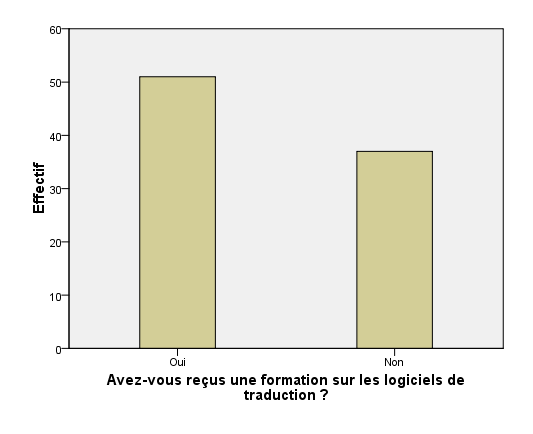
\includegraphics[width=0.6\textwidth]{fig01.png}
\caption{formation sur les logiciels de traduction.}
\label{fig01}
\source{d’après l’auteur.}
\end{figure}

En réponse à une autre question, la majorité très signifiante des répondantes (97.7\%) confirme l’utilité des logiciels de traduction comme on peut le voir dans la \Cref{fig02}:
\begin{figure}[htbp]
\centering
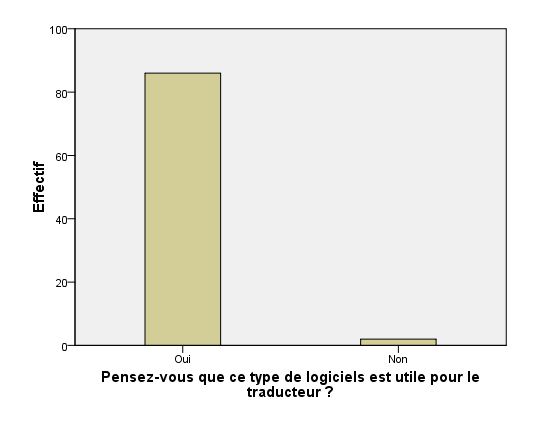
\includegraphics[width=0.6\textwidth]{fig02.png}
\caption{Importance des logiciels de traduction.}
\label{fig02}
\source{d’après l’auteur.}
\end{figure}

La \Cref{fig03} confirme les réponses de la question précédente puisque 86 répondantes (soit 97.7\%) confirme avoir utilisé des outils d’aide à la traduction et que 2 répondantes seulement ne les utilisent pas:
\begin{figure}[htbp]
\centering
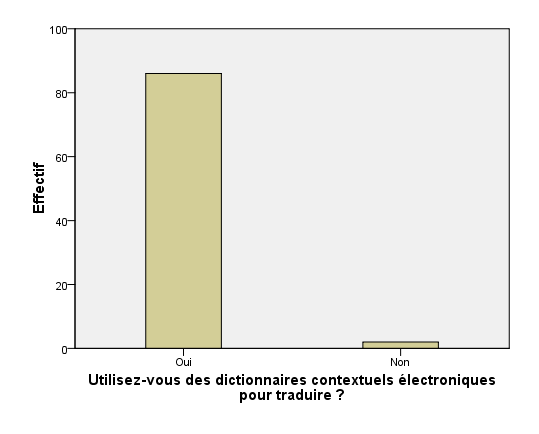
\includegraphics[width=0.6\textwidth]{fig03.png}
\caption{Utilisation des logiciels de traduction.}
\label{fig03}
\source{d’après l’auteur.}
\end{figure}

La \Cref{fig04} résume les réponses de la question: dans quels types de texte utilisez-vous les dictionnaires contextuels électroniques:
\begin{figure}[htbp]
\centering

\includegraphics[width=0.6\textwidth]{fig04.png}
\caption{Type de texte.}
\label{fig04}
\source{d’après l’auteur.}
\end{figure}

Les résultats confirment que 4 étudiantes utilisent les dictionnaires contextuels électroniques pour traduire des textes littéraires, 9 pour les textes techniques, 5 pour les textes économiques, 3 pour les textes politiques alors que la majorité soit 67 répondantes (76.1\%) utilisent les outils d’aides à la traduction pour tous les types.
\begin{figure}[htbp]
\centering
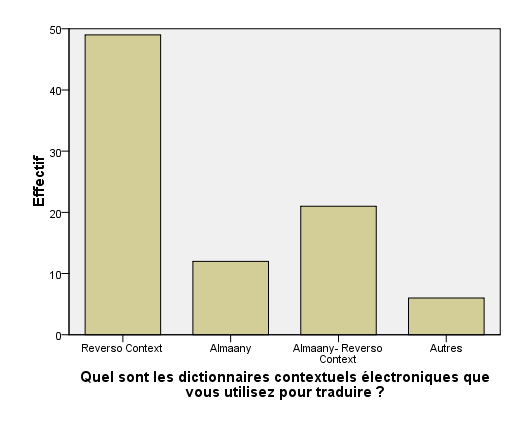
\includegraphics[width=0.6\textwidth]{fig05.png}
\caption{Dictionnaire contextuels électroniques.}
\label{fig05}
\source{d’après l’auteur.}
\end{figure}

Dans la \Cref{fig05}, nous remarquons que 49 étudiantes (soit 55.7\%) utilisent Reverso Context seulement et que 12 étudiantes (soit 13.6\%) utilisent Almaany seulement, alors que 21 répondantes (soit 23.9\%) combinent les deux logiciels. Les autres participantes (6 répondantes), font appel à d’autres applications.
\begin{figure}[htbp]
\centering
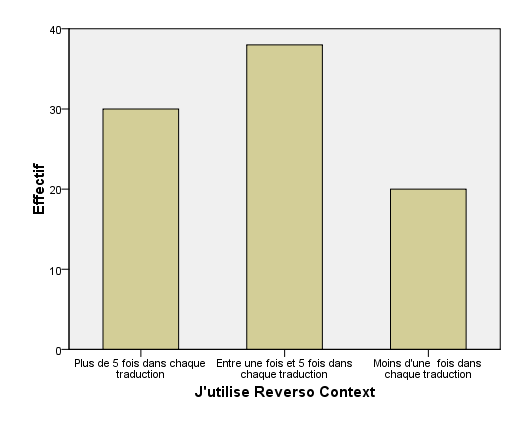
\includegraphics[width=0.6\textwidth]{fig06.png}
\caption{Utilisation de Reverso Context.}
\label{fig06}
\source{d’après l’auteur.}
\end{figure}

Dans la même optique, la \Cref{fig06} montre que la fréquence d’utilisation de Reverso Context n’est pas la même pour tous les étudiantes. 30 étudiantes (soit 34.1\%) ont recours au logiciel plus de 5 fois dans chaque traduction, 38 étudiantes (soit 43.2\%) l’utilisent moins de 5 fois dans chaque traduction alors que 20 étudiantes (22.7\%) l’utilisent moins d’une fois dans chaque traduction.
\begin{figure}[htbp]
\centering
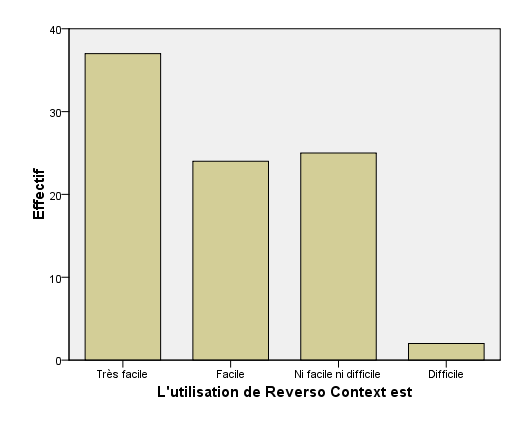
\includegraphics[width=0.6\textwidth]{fig07.png}
\caption{Difficulté de Reverso Context.}
\label{fig07}
\source{d’après l’auteur.}
\end{figure}

Comme on peut le constater dans la \Cref{fig07}, la majorité des répondantes n’a pas de problèmes d’utilisation avec Reverso Context puisque 37 étudiantes (42\%) le trouve très facile à utiliser, 24 (27.3\%) le trouve facile, 25 étudiantes sont neutres et seulement 2.3\% (soit 2 étudiantes) pensent qu’il est difficile à utiliser.
\begin{figure}[htbp]
\centering
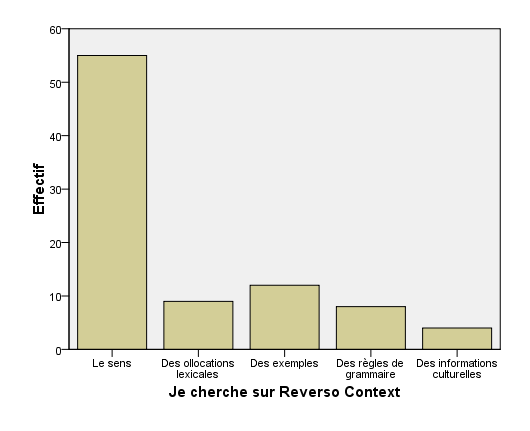
\includegraphics[width=0.6\textwidth]{fig08.png}
\caption{Type d’informations sur Reverso Context.}
\label{fig08}
\source{d’après l’auteur.}
\end{figure}

Selon la \Cref{fig08}, 80 participantes (soit 90.9\%) utilisent Reverso Context pour résoudre des problèmes relatifs au sens, alors que 8 participantes (soit 9.1\%) le font pour vérifier la langue. 
\begin{figure}[htbp]
\centering
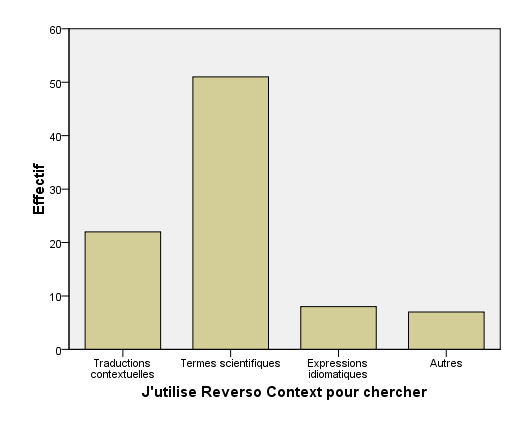
\includegraphics[width=0.6\textwidth]{fig09.png}
\caption{Type d’information sur Reverso Context.}
\label{fig09}
\source{d’après l’auteur.}
\end{figure}

Selon la \Cref{fig09} on constate que lorsqu’elles utilisent Reverso Context pour trouver le sens, 22 étudiantes (soit 25\%) l’utilisent en quête de traductions générées dans différents contextes. La majorité des répondantes (soit 58\%) font appel à ce logiciel pour résoudre des problèmes terminologiques. Pour 9.1\% des participantes, Reverso Context sert d’outil pour trouver des équivalents aux expressions idiomatiques.
\begin{figure}[htbp]
\centering
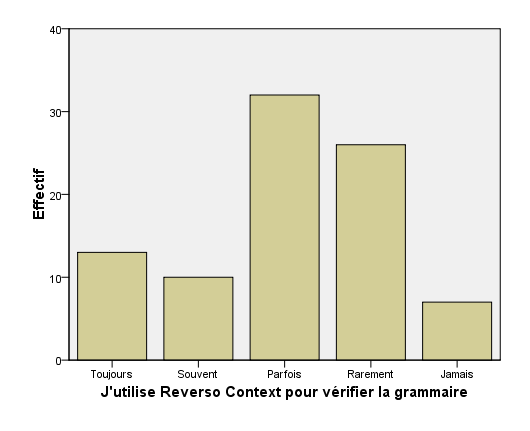
\includegraphics[width=0.6\textwidth]{fig10.png}
\caption{Reverso Context et la vérification grammaticale.}
\label{fig10}
\source{d’après l’auteur.}
\end{figure}

Dans la même optique de la \Cref{fig08}, la \Cref{fig10} montre que, bien que les logiciels de traduction ne fassent pas partie du cursus de la moitié des participants (42\%) comme on vient de le voir plus haut, la majorité des étudiants (97.7\%) non seulement pensent que ce type de logiciels est utile pour la traduction mais l’intègrent pour accomplir leurs tâches. Ceci croise les résultat d’une étude précédente \cite{bedjaoui2021} ou 86\% des enquêtés ont un recours systématique à la machine. En effet, les outils d’aide à la traduction tels que Reverso Context permettent d’accélérer le processus tout en participant à la réduction des coûts \cite{kehu2020}.

 L’étude a montré aussi que les étudiantes ont une préférence pour Reverso Context que tout autre logiciel. Elles font appel à ce logiciel pour traduire des textes relevant de domaines différents, soit pour rendre le sens soit pour assurer l’acceptabilité linguistique du texte cible. La linguistique de corpus, sous forme de banques de données linguistiques, des corpus, parallèles ou monolingues, dont se sert la traduction automatique en général et Reverso Context en particulier, pour donner accès à des traductions générées dans des contextes différents \cite{loock2016} explique ce choix. En effet, Reverso Context utilise des mémoires de traduction permettant un stockage et une recherche, très efficaces et rapide des textes existants sur support électronique, disponibles pour des langues variées, annotés avec des informations linguistiques, afin de permettre à la machine des interprétations conformes aux attentes des utilisateurs \cite{kehu2020}.
 
 \subsection{Etude qualitative}\label{sec-qualitative}
 
 Le premier texte que les étudiantes ont été amenées à traduire est un texte juridique qui relève plus précisément du Droit des Affaires (droit privé). La première phrase du texte concerne le domaine du Droit et il s’agit en vérité d’une définition générale. Pour la phrase: Le droit commercial est le droit applicable aux professionnels commerçants, aux entreprises commerciales et à certaines entreprises civiles non commerciales, nous sommes face à trois traductions assez différentes. Dans un premier exemple:
  
'\textlang{arabic}{ينطبق القانون التجاري على المهنيين التجار والمؤسسات التجارية والمدنية ولا غير التجارية}'.

L’étudiante, dans cet exemple, a opté pour la forme active. Tout en transposant littéralement le mot applicable, cette traduction prend en considération le sens des mots, leur contexte, mais elle n’est pas tout à fait fidèle dans la mesure où elle a «déforméle texte source en procédant à un «appauvrissement qualitatif» \cite{berman1984} à travers l’omission d’un mot, ce qui a affecté le sens. Nous remarquons que l’adjectif indéfini «certaines» n’a pas été traduit, et nous insistons sur l’importance de chaque mot quand il s’agit d’un texte juridique ou d’une définition. Les spécificités d’un tel texte exigent qu’on soit rigoureux avec chaque mot. Aussi observons-nous une légère modification qui opère une distinction qui n’existe pas dans le texte originel, c’est-à-dire en Français. En traduisant l’expression «certaines entreprises civiles non commerciales», l’étudiante a distingué entre entreprises civiles et entreprises non commerciales. La remarque que nous pourrions formuler est que cette distinction n’a pas lieu d’être, étant donné qu’il s’agit dans le texte d’entreprises civiles non commerciales.  Quant aux deux autres traductions, les deux étudiantes ont choisi d’adopter en arabe une forme du Français qui répond aux exigences définitoires des concepts en structurant la phrase selon cet ordre: syntagme nominal + syntagme verbal. Cette structure répond plus à la fonction du texte, c’est-à-dire la définition et nous évite aussi tout «ethnocentrisme» \cite{berman1984}. Toutefois, la fluctuation terminologique est perceptible à travers l’hésitation entre société et entreprise dans la traduction (2):

'\textlang{arabic}{القانون التجاري هو القانون المطبق على التجار المهنيين والشركات التجارية وبعض المؤسسات المدنية الغير تجارية}'.

Cet exemple de traduction montre que l’étudiante ne maîtrise pas assez le vocabulaire juridique, puisque le terme d’usage dans les textes de loi est bien évidemment «société». Or, les étudiantes semblent confondre «société» et «entreprise». En examinant de très près les différentes traductions, il est plausible de constater que l’ordre de mots pose constamment problème si bien qu’il fallait faire en sorte que les logiciels de traduction prenant en compte la nature et la fonction d’un mot sont donc privilégiés. En effet, dans le texte originel, nous rencontrons la formulation: professionnels commerçants. Si l’on analyse grammaticalement cette expression, nous remarquerons qu’il s’agit d’un groupe nominal étendu composé d’un nom (professionnels) enrichi d’un adjectif épithète (commerçant). Ainsi commerçants est un adjectif. Il est à conclure alors que l’exemple (1) de la traduction en arabe est le plus fidèle, puisque la traduction était plus fidèle en respectant cet ordre (nom + adjectif).  

'\textlang{arabic}{القانون التجاري هو القانون المطبق على التجار المهنيين على بعض المؤسسات التجارية وبعض المؤسسات المحلية الغير تجارية}'.

Le deuxième texte que les étudiantes avaient à traduire est un extrait du roman Le Conte de la Cigogne de \textcite{maza2017} comme nous l’avons déjà signalé. Pour des raisons méthodologiques, nous avons choisi de relever et d’analyser seulement quelques phrases seulement afin de pouvoir comparer les traductions générées respectivement par la TA et la TAO d’un côté et évaluer le produit final de l’autre côté. Dans ce contexte, les étudiantes ont procédé à une traduction purement automatique. Par la suite, elles sont intervenues pour modifier, changer ou corriger. Dans le souci d’assurer la commodité graphique de l’analyse, nous allons présenter à chaque fois une traduction par étudiante sous forme d’un tableau suivi d’un commentaire. Chaque tableau contiendra une partie pour la traduction de Reverso Context et une autre pour la traduction élaborée par le même logiciel sous le contrôle d’une étudiante.

Pour le premier extrait: Elle traînait sa jambe droite; Adnane m'a dit qu'elle avait eu une grosse infection et qu'elle avait été hospitalisée pendant plusieurs jours les traductions sont (\Cref{tbl01}):

\begin{table}[htpb]
\caption{Traduction du premier extrait.}
\label{tbl01}
\begin{tabularx}{\linewidth}{X|X}
\toprule 
TA & TAO \\
\midrule
\textlang{arabic}{تسحب ساقها اليمنى، وقد قال عدنان لي أنها كانت مصابة بعدوى كبيرة ويجب معالجتها بالمستشفى بضعة أيام.} & 
\textlang{arabic}{تجر ساقها اليمنى، وقد قال عدنان لي: أنها كانت مصابة بالتهاب في حالة متقدمة جداً. ونُقلت على الفور إلى المستشفى وظلت بضعة أيام. } \\
\bottomrule
\end{tabularx}
\source{d’après l’auteur.}
\end{table}

\textbf{Commentaire:} Dans cet exemple, l’étudiante a bien su choisir l’équivalent de traîner: \textlang{arabic}{جرّ} (Jarra\footnote{La transcription de l’arabe a été présenté dans étude menée par \cite{saadane2013}.} contrairement à Reverso qui a opté pour un verbe sémantiquement moins précis: \textlang{arabic}{سحب }( Sahaba) qui signifie faire aller dans une direction, avec force, quelque chose de lourd ou de résistant. De même, une erreur a été remarquée dans la traduction de «infection», la traduction automatique a choisi \textlang{arabic}{عدوى} (Àdwah) qui signifie une maladie ou une infection qui a été transmise et qui peut être transmise à une autre personne et dans le texte, l’écrivaine parle d’une infection due à une plaie mal soignée. Par contre, l’étudiante a pris cette notion en considération et a bien traduit le terme. Nous remarquons également que l’étudiante a bien préservé la forme passive dans la deuxième partie de la phrase. Mais en même temps elle a opté pour une structure plus au moins saccadée, contrairement à la version automatique, sans oublier les ajouts injustifiés: une expression \textlang{arabic}{على الفور} (Àlah al fawer) qui signifie immédiatement et une ponctuation (:). Pour cette dernière, il ne s’agit pas d’une ponctuation obligatoire qu’\textcite[p. 286]{berman1984} considère comme une déformation obligatoire du rythme due aux différences linguistiques, mais il s’agit d’un ajout erroné et non nécessaire.

Quant au deuxième extrait: Il avait travaillé très dur quand il était jeune. D'abord comme docker dans les docks de blé de la ville, ensuite comme camionneur. Il a parcouru tout le pays et a beaucoup d'histoires à raconter, mais il les raconte très peu, la traduction est (\Cref{tbl02}):

\begin{table}[htpb]
\caption{Traduction du deuxième extrait.}
\label{tbl02}
\begin{tabularx}{\linewidth}{X|X}
\toprule 
TA & TAO \\
\midrule
\textlang{arabic}{بدأ كعامل ميناء في موانئ القمح بالمدينة ثم كسائق شاحنة. سافر إلى جميع انحاء البلد ولديها الكثير من القصص تروى لكنه يسردها قليلا.} & 
\textlang{arabic}{فبدأ كعامل ميناء في حقول القمح هنا في المدينة، ثم عمل كسائق شاحنة وسافر كثيرا إلى جميع أنحاء البلاد ولديه الكثير من القصص ليرويها ٬ولكن لم يُخبر منها إلا القليل. } \\
\bottomrule
\end{tabularx}
\source{d’après l’auteur.}
\end{table}

\textbf{Commentaire:} Nous remarquons dans cet exemple que l’étudiante a respecté les exigences de la phrase arabe c’est-à-dire l’usage des conjonctions de coordination au lieu de la ponctuation et l’emploi de la forme active contrairement à Reverso qui a préservé la forme française. Nous pouvons dire qu’elle s’est servie de la traduction générée par la machine comme une piste pour fournir une traduction bien meilleure \cite{gile2005}. Ceci nous amène à observer un choix erroné pour la traduction de docker par \textlang{arabic}{عامل ميناء}  ‘quelqu’un qui travaille dans un port’. L’étudiante n’a pas effectué de recherche documentaire, et sa base de connaissance \cite{gile2005} ne contient pas d’information sur la localisation de la ville natale de l’écrivaine qui n’est pas une ville côtière et qui, par conséquent, n’est pas dotée d’un port. De son côté la traduction automatique était littérale et le contexte n’a pas été pris en considération.

Dans le troisième extrait :C’est intéressant de voir sur ces images comment l'action la plus noble de l'être humain rejoint son action la plus vile. Le graffiti n'est-il pas une célébration du mariage baroque entre l'art et le délit? La traduction est comme suit \Cref{tbl03}:

\begin{table}[htpb]
\caption{Traduction du troisième extrait.}
\label{tbl03}
\begin{tabularx}{\linewidth}{X|X}
\toprule 
TA & TAO \\
\midrule
\textlang{arabic}{من المثير للاهتمام رؤية في هذه الصور كيف انضم أنبل عمل للإنسان إلى عمله الأكثر سوء. هل الجرافيتي ليس هو احتفال بزفاف باروكي بين الفن والجريمة. ا.} & 
\textlang{arabic}{من المثير للاهتمام أن نرى مثل هذه الصور، وكيف يضم عمل الإنسان الأكثر نبلاً إلى عملهِ الأكثر فظاعة؟ أليست الرسومات على الجدران هي بمثابة احتفال بالزواج الباروك بين الفن        والجريمة؟. } \\
\bottomrule
\end{tabularx}
\source{d’après l’auteur.}
\end{table}

\textbf{Commentaire:} La traduction automatique était littéralement boiteuse: une structure inadéquate, un emprunt du mot graffiti, et l’usage du substantif au lieu du verbe pour traduire de voir. Pour ce dernier point, généralement un verbe à l’infinitif en français se traduit par le substantif dans la langue arabe mais la correction grammaticale dans cet exemple exige l’usage d’un autre verbe. D’ailleurs, l’étudiante a fait un choix réussi. Sa traduction est cohérente sauf pour l’emploi de la forme passive pour traduire rejoint, une erreur grammaticale dans l’accord de l’adjectif baroque et une mauvaise interprétation de la métaphore mariage baroque et l’étudiante et la machine n’ont pas compris qu’il s’agit d’une fusion artistiquement luxueuse entre l’art et le délit.

Pour le quatrième extrait: On peut dire qu'un graffiti est le lapsus de la société puisque c'est une brèchequi permet de la purgerdes idées interdites refouléesdans le subconscient collectif les résultats ont révélé les traductions suivantes \Cref{tbl04}:

\begin{table}[htpb]
\caption{Traduction du quatrième extrait.}
\label{tbl04}
\begin{tabularx}{\linewidth}{X|X}
\toprule 
TA & TAO \\
\midrule
\textlang{arabic}{ويمكن القول أن الجرافيتي هي هفوة المجتمع حيث أنها خرق يسمح بالقضاء على أفكار ممنوعة و مكبوتة في العقل الباطن للمجتمع.} & 
\textlang{arabic}{ويمكننا القول إن الرسومات الجدارية هي هفوة المجتمع حيث أنها الثغرة التي تتيح إعطاء فكرة ممنوعة ومكبوتة داخل العقل اللاواعي للمجتمع. } \\
\bottomrule
\end{tabularx}
\source{d’après l’auteur.}
\end{table}

\textbf{Commentaire:} Dans cet exemple, la machine a fourni une traduction relativement bien structurée puisque le texte évoque les traits d’un texte scientifique. Cependant, des erreurs d’ordre grammatical et sémantique ont été constatées: l’emploi de la préposition \textlang{arabic}{في} Fi au lieu de \textlang{arabic}{داخل} Dakhil qui signifie «à l’intérieur» et l’usage d’un mot signifiant le contraire de l’expression originelle en traduisant le mot purger par \textlang{arabic}{القضاء} (Qadaa) qui signifie l’élimination. De même, l’étudiante dans cet exemple a opté pour une transposition injustifiée pour traduire le mot idée (pluriel vers le singulier) et montre une faible maîtrise du vocabulaire de la psychologie ‘base de connaissances défaillante’ puisque le terme subconscient a été mal traduit par une association qui ne s’utilise pas souvent en arabe entre esprit et inconscient.

Quant au Cinquième extrait: Les auteurs de ces délits artistiques jugent eux-mêmes le thème qui les obsède comme indécent et choquant, les traductions sont (\Cref{tbl05}):

\begin{table}[htpb]
\caption{Traduction du cinquième extrait.}
\label{tbl05}
\begin{tabularx}{\linewidth}{X|X}
\toprule 
TA & TAO \\
\midrule
\textlang{arabic}{ويحكم مرتكبو هذه الجرائم الفنية أنفسهم على الموضوع الذي يملكهم بأنه غير لائق وصادم.} & 
\textlang{arabic}{ويرون أنفسهم واضعو هذه الجرائم الفنية والتي تثير اهتمامهم أن هذه الرسومات هي رسومات فاحشة وصادمة للمجتمع.} \\
\bottomrule
\end{tabularx}
\source{d’après l’auteur.}
\end{table}

\textbf{Commentaire:} La traduction automatique a fait du mot à mot et, contrairement à ce que nous pouvons penser, le résultat reste satisfaisant mais il est sémantiquement ambigu. De son côté l’étudiante a mal reformulé sa phrase mais le sens est représenté. Elle a aussi effectué des ajouts tels que \textlang{arabic}{مجتمع} (mojtamaa) ou société.
 
Pour le sixième extrait: Quand elle avait un moment de libre, elle tricotait, Elle portait tout le temps la même robe verte avec de grosses fleurs blanches, rouges et noires tout en bas, qui deviennent de plus en plus petites à mesure qu'on lève les yeux, jusqu'à ce qu'elles soient minuscules au col, les traductions sont (\Cref{tbl06}):

\begin{table}[htpb]
\caption{Traduction du sixième extrait.}
\label{tbl06}
\begin{tabularx}{\linewidth}{X|X}
\toprule 
TA & TAO \\
\midrule
\textlang{arabic}{وعندما كانت تملك وقت فراغ، كانت تحيك، كانت تلبس دائما نفس الفستان الأخضر بأزهار بيضاء وحمراء وسوداء في الأسفل والتي تصبح أصغر كلما رفعنا عينانا حتى تكون صغيرة جدا عند الياقة.} & 
\textlang{arabic}{وفي لحظات فراغها كانت تحيك مرتدية ذلك الفستان الأخضر المُشجّر بالزهور البيضاء والحمراء والسوداء في أسفل الفستان تتدرج تلك الزهور بالحجم وترتدي ذات الطوق أيضاً.} \\
\bottomrule
\end{tabularx}
\source{d’après l’auteur.}
\end{table}

\textbf{Commentaire:} Dans cet exemple le traitement automatique a bien fonctionné. A part quelques erreurs de ponctuation, la traduction est globalement plus satisfaisante par rapport à celle de l’étudiante. Cette dernière n’a pas utilisé une conjonction de coordination pour relier les deux parties de la phrase, elle a mal choisi l’équivalent de avec de grosses fleurs, et elle n’a pas précisé le degré de dégradation: en plus gros ou en plus petit. En outre s’est complètement trompée sur la dernière partie de la phrase. Nous estimons qu’une mauvaise méthode de travail a été adoptée. La difficulté est le résultat naturel d’un rapport non-adéquat entre la composante linguistique d’un texte et la compétence extralinguistique et méthodologique des étudiantes.

Les traductions du septième extrait, Elle s'était levée à 3h du matin au mois de Ramadhan pour préparer le shour (le petit-déjeuner avant le lever du soleil, sont (\Cref{tbl07}):

\begin{table}[htpb]
\caption{Traduction du septième extrait.}
\label{tbl07}
\begin{tabularx}{\linewidth}{X|X}
\toprule 
TA & TAO \\
\midrule
\textlang{arabic}{نهضت عند الثالثة صباحا في شهر رمضان لإعداد (الفطور قبل شروق الشمس).} & 
\textlang{arabic}{وكانت تعد وجبة السحور في الساعة الثالثة صباحاً من شهر رمضان قبل شروق الشمس.} \\
\bottomrule
\end{tabularx}
\source{d’après l’auteur.}
\end{table}

\textbf{Commentaire:} La traduction automatique est sémantiquement ambiguë, le logiciel n’a pas reconnu le mot s’hour ‘qui a été emprunté de l’arabe’ et n’a pas pris le co-texte en compte ‘le mot ramadan’, ni le contexte d’ailleurs, elle n’a donc pas fourni de traduction. Ce résultat confirme bien le manque du raisonnement logique expliqué plus haut. L’étudiante a bien reformulé sa phrase en omettant l’explication fournie par l’écrivaine et elle a comblé les lacunes culturelles puisqu’elle a pris le contexte en considération; elle s’adresse à une société musulmane qui connaît très bien ce type de repas. Le contenu doit impérativement être correct du point de vue informationnel et compatible du point du vue discursif. En tant que médiateur interculturel, le traducteur doit se garder de fournir, en opérant une quelconque explication, des éléments inexacts ou non vérifiés, induisant le lecteur en erreur au lieu de l’aiguiller vers la bonne interprétation du sens. Nous signalons que la traduction élaborée par l’étudiante n’est pas déformante ou annexionniste \cite{berman1984} puisque l’opération se déroule dans le cercle de la même culture ‘arabe’. Mais si le processus prenait le sens inverse (l’arabe vers le français) une traduction éthique qui reconnait et reçoit l’Autre en tant qu’Autre  serait sollicitée puisque le récepteur francophone a besoin de savoir que le S’hour  est le repas pris par les musulmans pendant le Ramadan et qu’il est différent du petit-déjeuner de point de vue heure et composition. 

Pour le huitième extrait: Elle devait traverser la cour pour atteindre la cuisine. Elle a préparé du couscous au sucre et aux raisins secs, a rempli l’assiette de couscous, et les verres de lait caillé et les a mis dans un plateau qu'elle devait porter à ses beaux-parents, Les traductions sont (\Cref{tbl08}):

\begin{table}[htpb]
\caption{Traduction du huitième extrait.}
\label{tbl08}
\begin{tabularx}{\linewidth}{X|X}
\toprule 
TA & TAO \\
\midrule
\textlang{arabic}{كان عليها أن تعبر الفناء للدخول إلى المطبخ. أعدت الكسكس بالسكر والزبيب وملأت  طبقا بالكسكس و أكوابا باللبن الرائب و وضعتهم في صينية يجب أن تحملها إلى حمويها.} & 
\textlang{arabic}{وكان عليها المرور بالفناء للدخول إلی المطبخ، فأخذت تعدّ الكسكس بالسكر والزبيب ملأت بهما الطبق، ثم أخذت تضع أكواب من الحليب الرائب في الصينية وفقا لأوامر والدي زوجها.} \\
\bottomrule
\end{tabularx}
\source{d’après l’auteur.}
\end{table}

\textbf{Commentaire:} L’étudiante a bien traduit la phrase en éliminant la ponctuation ‘remplacée par des conjonctions de coordination’ et a utilisé le contexte pour faire des choix sémantiques bien fondés, pour traduire lait caillé par exemple. Nous remarquons quand même un ajout injustifié à la fin de la phrase, une erreur grammaticale en rendant le mot couscous défini et un mauvais emploi de la dualité qui fait penser que là l’assiette a été remplie de raisin et de sucre.

\section{Résultats}\label{sec-resultados}
L’enquête a prouvé que les étudiantes ont tendance à utiliser les outils d’aide à la traduction en raison des différentes fonctionnalités qu’offre ce type de logiciels tel que Reverso Context. En effet, cet outil s’avère rapide et efficace grâce aux choix variés et multiples qu’il offre soit pour comprendre le sens et le rendre après ou pour assurer une version du texte cible conforme aux attentes et aux normes linguistiques des lecteurs cible.

De plus, l’analyse menée plus loin a démontré une réelle évolution pour la traduction automatique en matière de qualité de traduction: des traductions plus structurées, des choix plus riches et des champs lexicaux plus restreints. Dans ce contexte, Reverso se révèle être un outil offrant une multitude de combinaisons entre différentes langues et une riche mémoire de traduction contenant des traductions et des équivalences qui peuvent répondre aux besoins quotidiens des traducteurs qui travaillent sur des textes appartenant à des domaines assez disparates.

Cependant, l’automaticité de la traduction ne peut en aucun cas se passer de la supervision humaine avant, pendant et après l’opération traduisante. Le traducteur seul dispose de ce raisonnement logique grâce auquel il peut combiner des situations contextuelles concrètes, des structures syntaxiques adéquates et des règles grammaticales correctes pour bien interpréter le texte source et adapter le texte cible aux codes grammaticaux et sémantiques du public visé. Pour des raisons d’efficacité, une TA effectuée par un logiciel tel que Reverso Context doit être assistée par des compétences humaines assez solides. Nous parlons bien sûr d’un traducteur qui sait choisir ses outils et ses sources et qui dispose d’une base de connaissances suffisamment riche pour pouvoir faire la différence entre les différents contextes et prendre par la suite les décisions qui correspondent aux exigences de la qualité de traduction du texte en question.

Tenant compte de ces remarques, nous envisageons de développer des approches de traduction qui prennent en considération le contexte et le domaine auquel appartient le texte (juridique, économique, sociologique, etc.). Pour ce fait, il est indispensable d’élaborer des dictionnaires spécialisés (Arabe Français, Français-Arabe) qui seront intégrés comme des références de traduction contextuelle adoptant une approche basée sur l’utilisateur user- based qui prend en compte les besoins linguistiques et didactiques des étudiantes et des traducteurs \apud{zaretskaya2015}[p. 735]{schneider2019}. Dans cette optique, la reconnaissance des classes de mots est cruciale dans la mesure où elle est déterminante dans la traduction et le respect de l’ordre des mots. Force est de constater qu’il existe d’autres difficultés qui sont en rapport avec l’ordre des mots. Il ne s’agit pas à vrai dire d’exemples tirés des traductions, mais d’exemples que les étudiantes sont susceptibles de rencontrer. Pour nous limiter à une seule difficulté, nous mentionnons le cas des mots composés qu’il est possible de rencontrer dans d’autres textes. Ce problème de la traduction de mots composés a un lien bien entendu avec l’ordre des mots et la reconnaissance des catégories grammaticales. Dans le cas de la traduction de l’Arabe vers le Français ou vice-versa, le problème du pluriel et des catégories se pose avec acuité. En effet, le Français a d’autres difficultés à gérer, à savoir l’ordre des mots et le pluriel. La disposition des mots peut modifier le sens d’un composé. De plus, il faut respecter la place de l’adjectif et du nom qu’il enrichit. En Arabe, l’adjectif est placé toujours après le nom : dans les deux cas, le sens du composé reste le même. Quant au pluriel, il est source d’ambiguïtés en français. Il faut néanmoins être capable de dissocier les catégories grammaticales, car elles ne reçoivent pas les mêmes marques du pluriel : seuls les substantifs et les adjectifs ont une marque d’accord. Dans les mots composés, l’accord n’est pas toujours présent surtout dans des mots tels que \textit{Porte-manteau ou œil-de-bœuf}. Pour le premier mot au pluriel, seul le mot manteau prend la marque du pluriel, ce qui pourrait générer un problème de traduction automatique, notamment via ReversoContext. Pour le second mot, la difficulté est double, puisque le mot \textit{œil-de-bœuf}, selon le dictionnaire Larousse, a le sens de «Fenêtre, lucarne ronde ou ovale». Le traducteur automatique donne une traduction imprécise et inexacte en proposant le sens de trou ou serrure de la porte. Il en est de même pour la traduction de l’Arabe au Français. En effet, le traducteur automatique proposera d’autres mots en français et, souvent, une expression qui soit totalement déformée, sans tenir compte bien évidemment des règles de l’accord au pluriel des mots composés. En réalité, le mot composé \textit{œil-de-bœuf} déroge à la règle qui prescrit que le mot œil se décline en yeux au pluriel. Mais dans le cas du mot \textit{œil-de-bœuf}, l’accord au pluriel prévoit l’ajout d’un s, marque du pluriel seulement au mot œil, ce qui donne \textit{œils-de-bœuf}. À partir de cet exemple, nous soulignons le problème de traduction des prépositions, puisque certains mots composés contiennent des prépositions. Il est intéressant d’opérer quelques distinctions d’ordre sémantique et contextuel. Les prépositions doivent être spécifiées puisque dans les mots comme \textit{œil-de-bœuf}, \textit{cœur de lion, verre d’eau et verre à eau}, la valeur de la préposition n’est pas la même. Le premier mot est un mot composé, le second une périphrase verbale et les deux autres sont des mots composés contenant deux prépositions différentes qui affectent le sens. Si nous focalisons notre intérêt sur les deux derniers mots, il importe de formuler quelques remarques. La préposition «à» se distingue de la préposition de, car elle indique une fonction spécifique, alors que la préposition de marque la cohésion de référence entre les termes. Les expressions «un verre à eau» et «un verre d’eau» mettent bien en évidence les différences: le premier cas souligne la spécificité et l’utilisation que l’on fait du verre, alors que le second cas indique uniquement que le verre contient de l’eau. Les prépositions de et à sont les plus fréquentes dans la formation des composés. Aussi est-il important de bien les différencier. Les définitions exposées ci-dessus devraient permettre de préciser l’utilisation de chacune d’elles. Les autres prépositions intervenant en moindre mesure, leur interprétation sémantique semble moins pertinente.

\section{Conclusion}\label{sec-conclusoes}
En guise de conclusion, nous pouvons constater que Reverso Context est l’un des outils d’aide à la traduction les plus utilisés. Sa facilité ainsi que son corpus linguistique, varié et riche, permet aux étudiantes arabes de remédier à des problèmes de sens et de langue, leur permettant de produire des traductions plus au moins satisfaisantes.

Toutefois, les traducteurs automatiques comme Reverso Context rencontrent des problèmes touchant à plusieurs niveaux. Premièrement, le choix des mots en fonction de la spécialité comme nous l’avons soulevé à partir d’exemples de traduction. Parmi les difficultés auxquelles, nous avons eu affaire en recourant à la traduction automatique est celle de l’ordre des mots ‘les groupes nominaux étendus et la place des adjectifs. Enfin, le problème sémantique auquel il est important de trouver une solution est celui des mots composés contenant des prépositions. Le traducteur automatique doit reconnaître les classes grammaticales et, surtout, les expressions figées ‘les paraphrases’, les nuances contextuelles pour parvenir à traduire d’une manière efficace et réduire certaines erreurs citées subséquemment. 

Nous pouvons déduire aussi que le texte littéraire, comparé au texte scientifique, présente des caractéristiques linguistiques, stylistiques et culturelles très complexes quand il s’agit de traduction. Face à une situation pareille, la machine ne peut en aucun cas se passer de la supervision humaine avant, pendant et après l’opération traduisante. Seul le traducteur dispose de ce raisonnement logique grâce auquel il peut traduire des expressions idiomatiques des structures syntaxiques adéquates et des règles grammaticales correctes pour bien interpréter le texte source et adapter le texte cible aux codes grammaticaux, sémantiques et culturels du public visé.

Ainsi, pouvons-nous confirmer que la traduction automatique ne donnera point de traduction exemplaire et fidèle, mais fera bon guide à nos étudiantes. Elle peut se présenter comme une source de départ ouvrant des pistes vers des traductions plus correctes \cite{gile2005}.  A posteriori, il faut se mettre en tête que ce type de source peut être aussi un mauvais serviteur et l’on risque de se laisser influencer par les mots choisis et de se fourvoyer ainsi sur de fausses traductions \cite[p. 214]{aubin1995} puisque:
 
\begin{quote}La traduction automatique est un domaine extrêmement complexe car la signification des mots dépend du contexte dans lequel ils sont utilisés. La mise en place d’un service de traduction automatique rapide et efficace risque de prendre encore un certain temps. (GoogleTranslate TPSG, 2013).
\end{quote}

Dans la même perspective, nous envisageons d’orienter d’autres recherches vers le rôle que l’intelligence artificielle pourrait jouer dans d’autres domaines de la traduction notamment celui de la traduction audiovisuelle, pour répondre à des questions pertinentes et essentielles telles que: quels types de problèmes risque-t-on de rencontrer dans l’utilisation des techniques de l’intelligence artificielle dans le processus de la traduction audiovisulle?

\section{Acknowledgements}\label{sec-agradecimentos}
\begin{english}
\textit{
This research was funded by the Deanship of Scientific Research at Princess Nourah bint Abdulrahman University, through the Research Funding Program (\textbf{Grant No \#FRP -1440-6}).
I extend my appreciation to \textbf{Chaouki Bounaas} for his significant assistance and constructive comments. I would also like to thank the master's students \textbf{Mada El Saeed}, \textbf{Rafeef Al Olyan} and \textbf{Hayfa Almalki} for their enthusiasm and their application during the realization of this research project.
}
\end{english}

\printbibliography\label{sec-bib}
% if the text is not in Portuguese, it might be necessary to use the code below instead to print the correct ABNT abbreviations [s.n.], [s.l.] 
%\begin{portuguese}
%\printbibliography[title={Bibliography}]
%\end{portuguese}



\end{document}
